\documentclass[UTF8]{ctexart}
\usepackage{graphicx}
\title{\heiti 第一次离散数学作业}
\graphicspath{{figures/}}
\author{\kaishu 闫嘉明}
\date{\today}

\begin{document}
\maketitle
\part{1.1}
\section{20}
\subsection{(a)}
inclusive or

\subsection{(b)}
exclusive or

\subsection{(c)}
inclusive or

\subsection{(d)}
exclusive or

\section{33}
\subsection{(a)}
$$(p \vee q) \to (p \oplus q)$$
The truth table:\\

\begin{tabular}{|c|c|c|c|c|}
    \hline
    p & q & $p \vee q$ & $p \oplus q$ & $(p \vee q) \to (p \oplus q)$\\
    \hline
    T & T & T & F & F\\
    \hline
    T & F & T & T & T\\
    \hline
    F & T & T & T & T\\
    \hline
    F & F & F & F & T\\
    \hline
    
\end{tabular}
\section{35}
\subsection{(c)}
$$(p \to q)\vee (\neg p \to q)$$
The truth table:\\\\
\begin{tabular}{|c|c|c|c|c|}
    \hline
    p & q & $p \to q$ & $\neg p \to q$ & $(p \to q)\vee (\neg p \to q)$\\
    \hline
    T & T & T & T & T\\
    \hline
    T & F & F & T & T\\
    \hline
    F & T & T & T & T\\
    \hline
    F & F & T & F & F\\
    \hline
    
\end{tabular}
\part{1.2}
\section{9}
let p denotes "the system is in multiuser state".\\
let q denotes "the system is operating normally"\\
let a denotes "the kernel is functioning"\\
let b denotes "the system is in interrupt mode"\\
according to the description, we know:\\
$$p \Leftrightarrow q, q \rightarrow a, \neg a \oplus b, \neg p \rightarrow b$$\\
and b is false.\\
assume all propositons are true.\\
then $\neg a$ is true, a is false.\\
because $q\to a$ is true, so q is false.\\
because $p \Leftrightarrow q$, so p is false.\\
so $\neg p$ is true. so $\neg p \to b$ is false, which is contradict with the assumption.\\
so these system specifications are not consistent. 
\section{20}
let p denotes "The two of us are both knights"

let q denotes "A is a knave"

the truth table:

\begin{tabular}{|c|c|c|c|c|}
    \hline
    A & B & p & q & conclusion\\
    \hline
    knight & knight & true & false & wrong\\
    \hline
    knight & knave & false & false & wrong\\
    \hline
    knave & knight & false & true & right\\
    \hline
    knave & knave & false & true & wrong\\
    \hline
\end{tabular}

\textbf{so A is a knave and B is a knight.}
\section{34}
let a,b,c,d,e denote Kevin,Heather,Randy,Vijay,Abby is chatting.\\
according to the description:\\
$a\vee b,c \oplus d,e \to c,a \wedge d,\neg a \wedge \neg d,b\to a \wedge e$\\
if a is true, d is true, and c is false, so e is false, then $a \wedge e$ is false so b is false.\\
in another case, if a is false, d is false, and c is true, no matter e is true or false, $a \wedge e$ is false, so b is false. So $a \vee b$ is false, which contradict with the description. \\
\textbf{In conclusion, Kevin and Vijay are chatting, it's possible to determine who is chatting.}
\section{43}
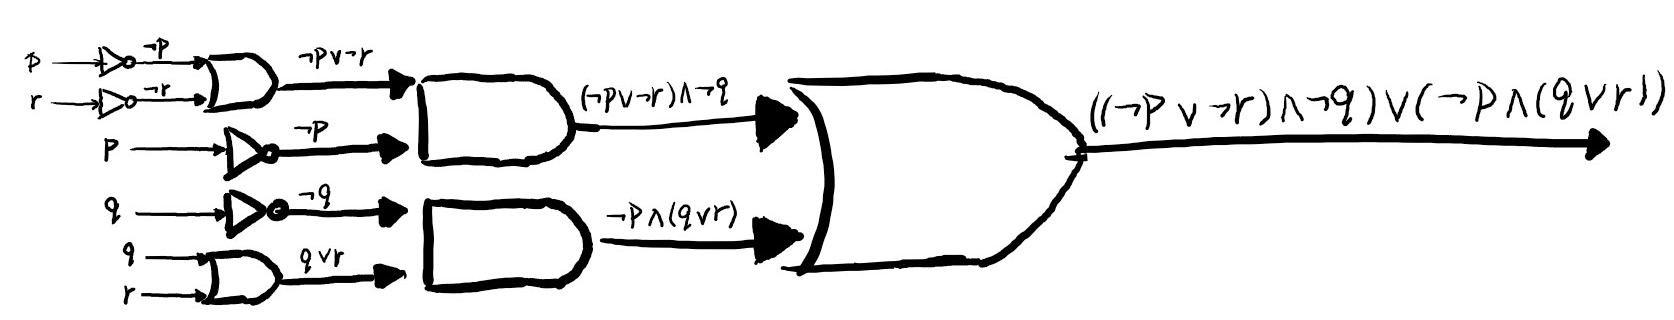
\includegraphics[scale=0.7]{homework1a}
\part{1.3}
\section{15}
$(\neg p \wedge (p \rightarrow q))\rightarrow \neg p$ is a tautology.\\
Assume $(\neg p \wedge (p \rightarrow q))\rightarrow \neg p$ is false, then $(\neg p \wedge (p \rightarrow q))$ is true while p is false.
however, if $(\neg p \wedge (p \rightarrow q))$ is true, then $\neg q and p \rightarrow q$ is true. Then, q is false. And because $p \rightarrow q$ is true and q is false, p is false. So $\neg p$ is true, which contradicts with the assumption.\\
\textbf{In conclusion: $(\neg p \wedge (p \rightarrow q))\rightarrow \neg p$ is a tautology.}
\section{23}
If $(p \rightarrow r)\wedge (q\rightarrow r)$ is true, then $(p \rightarrow r) and (q\rightarrow r)$ are true. So $(p\vee q)\rightarrow r$ is true.

If $(p \vee q)\rightarrow r$ is false, then $p \vee q$ is true and r is false. Then p and q are not false at the same time. So $(p \rightarrow r)\wedge (q\rightarrow r)$ is false.\\
$(p \rightarrow r)\wedge (q\rightarrow r)$ and $(p \vee q)\rightarrow r$ are of the same value. \textbf{In conclusion, they are logically equivalent.}
\section{45}
Given a compound proposition p, form its truth table and write a proposition q in disjunctive normal form that is logically equivalent to p. q invloves only $\neg,\wedge and \vee$, so these three operators form a functionally complete set. 
Then according to De Morgen's law, we can replace the operator $\wedge$ with $\vee and \neg$. So $\vee and \neg$ form a functionally complete set. 
\end{document}